\section{gufi\_dir2index}

\subsection{Outline}
gufi\_dir2index is used in order to turn a directory into a GUFI index. This process involves creating a database template that will be copied and modified for all directories and sub-directories as gufi descends down the tree. The information of the non-directories is stored inside of the databases. Permissions are established and any resulting errors establishing them are ignored

\subsection{Flags}

\begin{table} [h]
\centering
\begin{tabular}{l|r}
Flag & Functionality \\\hline
-h & help manual \\
-H & Show assigned input values \\
-n \textless num\_threads\textgreater  & define number of threads to use \\
-x & pull xattrs from source file-sys into GUFI \\
-z \textless max\_level\textgreater & maximum level to go down to
\end{tabular}
\caption{\label{fig:Flags_for_dir2index}Flags and Arguments}
\end{table}

\begin{figure} [h]
\centering
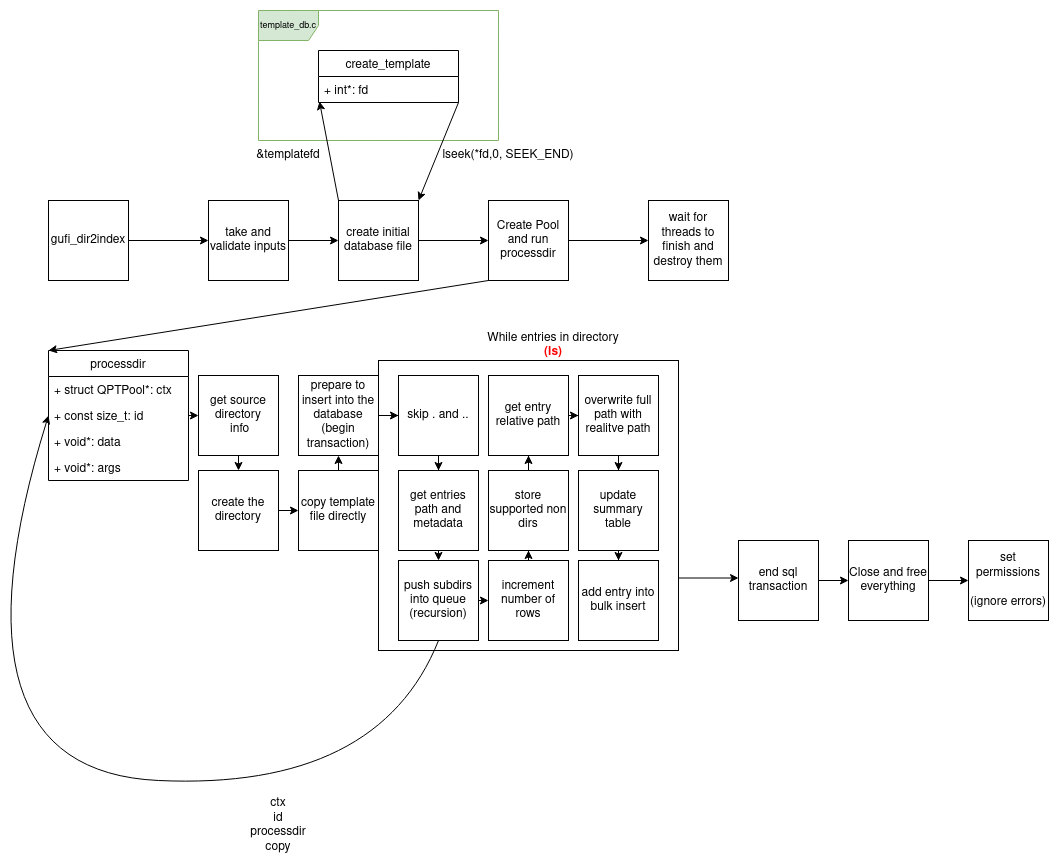
\includegraphics[width=1.0\textwidth]{images/gufi_dir2index.png}
\caption{\label{fig:gufi_dir2index}gufi\_dir2index workflow}
\end{figure}

\subsection{Usage}
\texttt{gufi\_dir2index [flags] [directory to index] [location to place indexed directory]}


